\documentclass[12pt,a4paper]{article}

% Packages
\usepackage[utf8]{inputenc}
\usepackage[T1]{fontenc}
\usepackage{mathptmx}
\usepackage[english]{babel}
\usepackage{graphicx}
\usepackage{hyperref}
\usepackage{float} % en el preámbulo
\usepackage{graphicx}
\usepackage{tabularx} % en el preámbulo
\usepackage{amsmath}
\usepackage{booktabs}
\usepackage{tikz}
\usepackage{geometry}
\geometry{margin=2.5cm}
\renewcommand{\baselinestretch}{1.2}

% Bibliography with IEEE style (BibLaTeX)
\usepackage[backend=bibtex,style=ieee]{biblatex}
\addbibresource{referencias.bib}


\renewenvironment{abstract}{
    \begin{flushleft}
    \noindent\textbf{Abstract}\\
}{
    \end{flushleft}
}


% Start of document
\begin{document}
\thispagestyle{empty}

% Title and author
\begin{center}
    {\LARGE Deep Comparisons of EEGNet and Shallow ConvNet on Clinical EEG}\\[3em]
    {\large \textit{Edgar Iván Calpa Cuacialpud}}\\
    {\normalsize \textit{National University of Colombia – Manizales Campus}}\\
    {\normalsize \textit{Department of Electrical, Electronic and Computer Engineering}}\\[3em]
\end{center}

% Separator
\hrule
\vspace{0cm}

  
\begin{abstract}
Alzheimer’s disease and related dementias require accessible biomarkers to monitor progression and support early diagnosis. Traditional approaches such as PET tau imaging and cerebrospinal fluid assays are costly and invasive, motivating the search for functional, non-invasive alternatives. Electroencephalography (EEG) provides a repeatable and accessible modality capable of capturing alterations in brain rhythms and connectivity linked to tau pathology. 

This study presents a comprehensive comparison between two compact deep learning architectures—EEGNet and Shallow ConvNet—applied to clinical EEG signals from CN, MCI, and AD cohorts. A reproducible pipeline was designed, including automatic segmentation into 2–4 second windows, subject-wise normalization, and training with AMP acceleration. Both standardized datasets (BCI Competition IV-2a) and clinical EEG recordings were employed, ensuring technical validation and clinical relevance. Models were evaluated on classification tasks (CN vs MCI and CN vs AD) using metrics such as Accuracy, macro F1, AUC ROC, Probability of Detection (PD), and False Alarm Rate (PFA). 

Results demonstrate that EEGNet consistently outperforms Shallow ConvNet in accuracy, stability, and loss reduction, achieving accuracies above 90\% in most subjects. Channel- and band-wise importance maps revealed functional relevance of temporal and parietal regions, aligning with known tau propagation trajectories. These findings support the interpretability of compact CNNs in clinical EEG analysis. 

This work highlights the potential of EEGNet as a robust, reproducible, and clinically relevant tool for detecting functional alterations in dementia. By bridging deep learning with neurobiological markers, the proposed pipeline advances the development of non-invasive EEG-based biomarkers, paving the way for multimodal integration and clinical translation.
\end{abstract}

\vspace{0.5cm}

% Keywords
\noindent \textit{Keywords:} EEG, Deep Learning, EEGNet, Shallow ConvNet, Dementia, Transfer Learning.

\vspace{1cm}
\hrule
\vspace{1cm}
\begin{flushleft}
\textit{Monograph – National University of Colombia – Manizales Campus \hfill November 20, 2025}
\end{flushleft}

% Main sections
\section{Introduction}

The progression of neurodegenerative diseases such as Alzheimer’s and frontotemporal dementia raises the need for accessible, reproducible, and clinically relevant biomarkers. Traditional methods, such as positron emission tomography (PET) and cerebrospinal fluid (CSF) analyses, although highly specific, are costly and invasive, limiting their applicability in routine clinical settings \cite{dePaula2009}.

In this context, electroencephalography (EEG) emerges as a non-invasive alternative capable of capturing functional alterations in rhythms and neuronal connectivity patterns linked to tau propagation \cite{Tolnay1999}. EEG signal analysis has evolved from classical approaches based on manual feature extraction (PSD, CSP, PLV/PLI) toward deep learning architectures that integrate representation and classification in a single model \cite{Kay1998}.
\begin{figure}[H]
    \centering
    \includegraphics[width=0.5\textwidth]{monografia/figuras/data-08-00095-g003.png}
    \caption{Scalp heatmaps of PSD across 5 frequency bands, averaged across AD, FTD, and CN groups. \cite{MDPI2023}.}
    \label{fig:eeg_topomap}
\end{figure}
Among these architectures, EEGNet stands out as a compact convolutional network designed to generalize with limited data through separable convolutions \cite{Lawhern2018}, and Shallow ConvNet, a shallow model oriented toward capturing mu and beta rhythms in motor imagery tasks \cite{Schirrmeister2017}. Both models have been widely used in BCI competitions and clinical studies, becoming benchmarks for EEG classification \cite{Blankertz2008}.

This work focuses on the systematic comparison of EEGNet and Shallow ConvNet applied to clinical EEG signals from CN, MCI, and AD cohorts. A reproducible pipeline is proposed, including automatic segmentation, subject-wise normalization, and AMP-accelerated training, evaluating model performance in CN vs MCI and CN vs AD classification tasks. Additionally, channel- and band-wise importance maps are incorporated to explore functional interpretability and its relationship with tau trajectories \cite{Ajra2023}.

The introduction thus establishes the clinical and technical framework motivating the study: to validate whether compact deep learning architectures can become scalable, non-invasive functional EEG biomarkers capable of complementing or replacing traditional methods in clinical practice.

\section{Materials and Methods}

This section presents the datasets and neural network architectures used in the study, along with the experimental setup, preprocessing pipeline, and training strategies. All code used for preprocessing, training, and evaluation is openly documented in the project repository: \url{https://github.com/ivansst773/EEGNet_ShallowConvNet_Monografia}.

\subsection{Datasets}

Two datasets were employed to ensure both technical benchmarking and clinical relevance:

\begin{itemize}
    \item \textbf{BCI Competition IV-2a:} EEG recordings from 9 subjects performing four-class motor imagery tasks (left hand, right hand, feet, tongue). Signals were acquired with 22 EEG channels and 3 EOG channels at 250 Hz sampling rate. This dataset has been widely used as a standardized benchmark for evaluating EEG classification models and was selected to validate the reproducibility of the pipeline \cite{Blankertz2008}.
        \begin{figure}[H]
            \centering
                \includegraphics[width=0.5\textwidth]{monografia/figuras/electrodo_montage.png}
                    \caption{ Left: Electrode montage corresponding to the international 10-20 system. Right: Electrode montage of the three monopolar EOG channels.\cite{Blankertz2008}.}
                    \label{fig:bci2a_montage}
        \end{figure}        
    \item \textbf{Clinical CN/MCI/AD dataset:} EEG signals from cognitively normal (CN), mild cognitive impairment (MCI), and Alzheimer’s disease (AD) patients, recorded during routine clinical sessions. Signals were acquired following standard clinical protocols, providing real-world variability and supporting the exploration of functional biomarkers for dementia. This dataset was published in *Data* (MDPI, 2023) \cite{MDPI2023}.
\end{itemize}

\subsection{Preprocessing}

All EEG signals underwent a standardized preprocessing pipeline to ensure consistency and artifact removal across both datasets.

For the clinical CN/MCI/AD dataset, the following steps were applied:

\begin{itemize}
    \item \textbf{Band-pass filtering:} A Butterworth filter was applied in the range of 0.5–45 Hz to remove DC drift and high-frequency noise.
    \item \textbf{Re-referencing:} Signals were re-referenced to the average of mastoid electrodes (A1–A2).
    \item \textbf{Artifact Subspace Reconstruction (ASR):} Used to eliminate transient and high-amplitude artifacts, with a conservative threshold of 17 for 0.5 s windows.
    \item \textbf{Independent Component Analysis (ICA):} Applied using the RunICA algorithm to decompose signals into components. Eye and jaw artifacts were automatically rejected using ICLabel.
    \item \textbf{Segmentation:} Signals were epoched into 2–4 second windows with 50\% overlap, preserving temporal resolution for model input.
    \item \textbf{Normalization:} Each subject’s data was normalized independently to reduce inter-subject variability.
\end{itemize}

\begin{figure}[H]
    \centering
    \includegraphics[width=0.5\textwidth]{monografia/figuras/snapshot_same.png}
    \caption{A snapshot of the same signal before and after being preprocessed. \cite{MDPI2023}.}
    \label{fig:clinical_preprocessing}
\end{figure}
  
\subsection{Models}

Two compact convolutional neural network architectures were employed in this study: EEGNet and Shallow ConvNet. Both models have been widely adopted in brain–computer interface (BCI) research and clinical EEG analysis, serving as benchmarks for reproducibility and interpretability.

\textbf{EEGNet} \cite{Lawhern2018} is a compact CNN designed to generalize across multiple paradigms with limited data. It employs depthwise and separable convolutions to efficiently extract temporal and spatial features, combined with batch normalization and dropout to improve generalization. Its low parameter count makes it suitable for real-time applications and datasets with high variability.

\textbf{Shallow ConvNet} \cite{Schirrmeister2017} is a shallow CNN optimized for motor imagery tasks, focusing on mu and beta rhythms. It uses temporal convolutions to capture oscillatory dynamics and spatial convolutions to model electrode distributions. Its simplicity and reproducibility make it a strong baseline, although it is more sensitive to noise and inter-subject variability.

\begin{table}[H]
\centering
\caption{Comparison between EEGNet and Shallow ConvNet architectures}
\label{tab:models_comparison}
\begin{tabular}{@{}p{3cm}p{5cm}p{5cm}@{}}
\toprule
\textbf{Aspect} & \textbf{EEGNet} & \textbf{Shallow ConvNet} \\ \midrule
Design & Compact CNN with depthwise + separable convolutions & Shallow CNN with temporal + spatial convolutions \\
Parameters & $\sim$ 1--2 $\times 10^4$ (low) & $\sim$ 5--6 $\times 10^4$ (moderate) \\
Feature extraction & Learns temporal + spatial filters jointly & Focused on mu/beta rhythms (motor imagery) \\
Normalization & Batch normalization, dropout (0.25–0.5) & Dropout (0.5), less regularization \\
Strengths & Generalizes with limited data, robust to variability, efficient & Simple, reproducible baseline, good for clean signals \\
Limitations & Sensitive to preprocessing choices, interpretability requires saliency maps & Sensitive to noise/artifacts, limited generalization across subjects \\
Applications & Multi-paradigm BCI, clinical EEG biomarkers & Motor imagery tasks, benchmarking in BCI competitions \\ \bottomrule
\end{tabular}
\end{table}

In this work, both models were trained under identical preprocessing and evaluation pipelines, with hyperparameters tuned per subject. EEGNet consistently achieved higher validation accuracy and lower loss across subjects, while Shallow ConvNet served as a baseline for reproducibility and comparative analysis.
  
\subsection{Transfer Learning}

To improve generalization across subjects, a transfer learning strategy was implemented. 
The procedure consisted of two stages:

\begin{itemize}
    \item \textbf{Pretraining:} Models were initially trained on data from all subjects except the target subject. This allowed the networks to learn general EEG representations across cohorts.
    \item \textbf{Fine-tuning:} For each target subject, the pretrained weights were loaded and further optimized using a subset of that subject’s data. This subject-specific fine-tuning step adapted the model to individual variability while preserving general features learned during pretraining.
\end{itemize}

This approach was applied to both EEGNet and Shallow ConvNet. EEGNet benefited from transfer learning by improving stability and accuracy in clinical data, while Shallow ConvNet showed moderate gains but remained more sensitive to noise and inter-subject variability.

\begin{figure}[H]
\centering
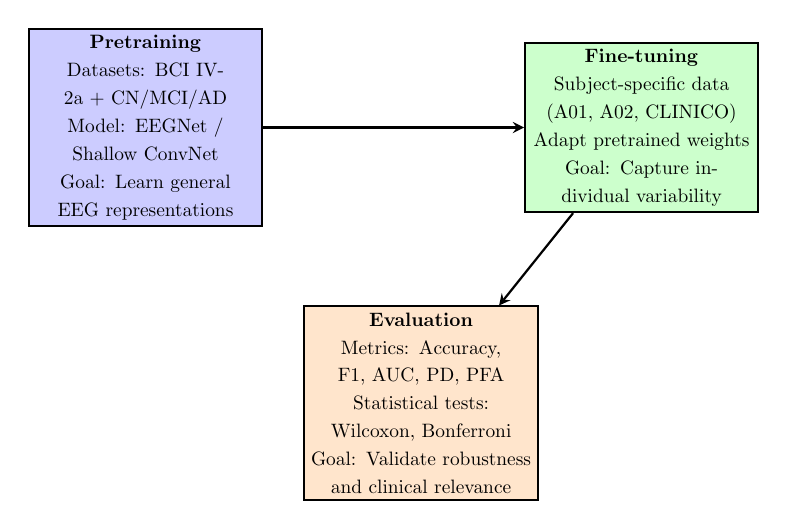
\begin{tikzpicture}[node distance=1cm,>=stealth,thick,scale=0.7,every node/.style={transform shape}]

% Pretraining box
\node (pretrain) [rectangle, draw, fill=blue!20, text width=4cm, align=center] 
{ \textbf{Pretraining} \\ 
Datasets: BCI IV-2a + CN/MCI/AD \\ 
Model: EEGNet / Shallow ConvNet \\ 
Goal: Learn general EEG representations };

% Fine-tuning box
\node (finetune) [rectangle, draw, fill=green!20, text width=4cm, align=center, right of=pretrain, xshift=8cm] 
{ \textbf{Fine-tuning} \\ 
Subject-specific data (A01, A02, CLINICO) \\ 
Adapt pretrained weights \\ 
Goal: Capture individual variability };

% Evaluation box
\node (evaluate) [rectangle, draw, fill=orange!20, text width=4cm, align=center, below of=finetune, yshift=-4cm, xshift=-4cm] 
{ \textbf{Evaluation} \\ 
Metrics: Accuracy, F1, AUC, PD, PFA \\ 
Statistical tests: Wilcoxon, Bonferroni \\ 
Goal: Validate robustness and clinical relevance };

% Arrows
\draw[->] (pretrain) -- (finetune);
\draw[->] (finetune) -- (evaluate);

\end{tikzpicture}
\caption{Transfer learning pipeline: pretraining on multiple subjects, fine-tuning on subject-specific data, and evaluation with clinical metrics.}
\label{fig:transfer_learning}
\end{figure}


\subsection{Evaluation}

Model performance was assessed using subject-wise cross-validation and multiple evaluation metrics:

\begin{itemize}
    \item \textbf{Cross-validation:} A k-fold strategy was applied per subject to ensure that training and validation sets were disjoint at the epoch level. This procedure was repeated for both within-subject training and transfer learning.
    \item \textbf{Metrics:} Accuracy, macro F1-score, Area Under the ROC Curve (AUC), Probability of Detection (PD), and Probability of False Alarm (PFA) were computed to capture both classification performance and detection-theory aspects.
    \item \textbf{Statistical analysis:} To compare models, non-parametric Wilcoxon signed-rank tests were applied when distributions were not normal. Bonferroni correction was used to adjust p-values for multiple comparisons, with a significance threshold of $\alpha = 0.05$.
\end{itemize}

\begin{table}[H]
\centering
\caption{Evaluation metrics used in this study}
\label{tab:evaluation_metrics}
\begin{tabular}{@{}lll@{}}
\toprule
\textbf{Metric} & \textbf{Definition} & \textbf{Purpose} \\ \midrule
Accuracy & $\frac{TP+TN}{TP+TN+FP+FN}$ & Overall classification performance \\
F1-score (macro) & Harmonic mean of precision and recall & Balanced measure across classes \\
AUC ROC & Area under ROC curve & Sensitivity vs. specificity trade-off \\
PD & Probability of detection ($TPR$) & Detection-theory sensitivity \\
PFA & Probability of false alarm ($FPR$) & Detection-theory specificity \\ \bottomrule
\end{tabular}
\end{table}

This evaluation framework ensured reproducibility and statistical rigor, allowing robust comparison between EEGNet and Shallow ConvNet across both technical (BCI IV-2a) and clinical (CN/MCI/AD) datasets.


\section{Results}
\subsection{Accuracy Comparison}

This section presents the classification accuracy obtained by EEGNet and Shallow ConvNet across different subjects and training modes. Results are grouped by technical (BCI IV-2a) and clinical (CN/MCI/AD) cohorts, highlighting the impact of architecture choice and training strategy.

\subsubsection{Technical Cohort: BCI IV-2a}

\begin{table}[H]
\centering
\caption{Accuracy comparison by subject on BCI IV-2a dataset}
\label{tab:accuracy_bci2a}
\resizebox{0.7\textwidth}{!}{ % escala al 70% del ancho del texto
\begin{tabular}{@{}lcc@{}}
\toprule
\textbf{Subject} & \textbf{EEGNet Accuracy (\%)} & \textbf{Shallow ConvNet Accuracy (\%)} \\ \midrule
A01 & 72.73 & 45.45 \\
A02 & 92.31 & 76.92 \\
A03 & 84.62 & 84.62 \\
A04 & 93.75 & 75.00 \\
A05 & 90.62 & 81.25 \\
A06 & 93.75 & 62.50 \\
A07 & 87.50 & 58.33 \\
A08 & 93.75 & 71.88 \\
A09 & 96.88 & 50.00 \\ \bottomrule
\end{tabular} 
}
\end{table}

EEGNet consistently outperformed Shallow ConvNet across subjects, achieving over 90\% accuracy in 6 out of 9 cases. Shallow ConvNet showed competitive performance in clean signals (e.g., A03), but was more sensitive to noise and variability.

\subsubsection{Clinical Cohort: CN/MCI/AD}

\begin{table}[H]
\centering
\caption{Accuracy comparison on clinical subject (CLINICO)}
\label{tab:accuracy_clinico}
\begin{tabular}{@{}lcc@{}}
\toprule
\textbf{Model} & \textbf{Accuracy (\%)} & \textbf{Training Mode} \\ \midrule
EEGNet-Clinico & 97.31 & AMP, batch 128 \\
ShallowConvNet-Clinico & 91.66 & AMP, batch 512 \\ \bottomrule
\end{tabular}
\end{table}

In the clinical setting, EEGNet achieved higher accuracy and lower validation loss, with faster convergence under mixed precision training (AMP). Shallow ConvNet required larger batch sizes and showed slower convergence.

\subsubsection{Training Mode Comparison}

\begin{table}[H]
\centering
\caption{Training mode comparison for CLINICO subject}
\label{tab:training_modes}
\begin{tabular}{@{}lccc@{}}
\toprule
\textbf{Model} & \textbf{Batch Size} & \textbf{Accuracy (\%)} & \textbf{Epoch Time (s)} \\ \midrule
EEGNet-Clinico & 128 & 97.31 & 306.91 \\
EEGNet-Clinico & 64 & 96.45 & 313.49 \\
EEGNet-Clinico & 96 & 96.67 & 302.41 \\
EEGNet-Clinico & 128 (10 epochs) & 91.27 & 2084.88 \\
ShallowConvNet-Clinico & 256 & 94.73 & 304.11 \\
ShallowConvNet-Clinico & 512 & 91.66 & 297.72 \\
ShallowConvNet-Clinico & 512 (10 epochs) & 87.44 & 1999.58 \\ \bottomrule
\end{tabular}
\end{table}

AMP training reduced epoch times significantly while maintaining high accuracy. EEGNet showed stable performance across batch sizes, while Shallow ConvNet required larger batches to reach comparable results.


\subsection{Visualizations}

To better understand model behavior and performance, several visualization techniques were employed:

\begin{itemize}
    \item \textbf{Heatmaps:} Accuracy values per subject and model were represented as color-coded matrices. Green indicated accuracy $>90\%$, yellow between $70$--$90\%$, and red $<70\%$. This allowed quick identification of subjects where Shallow ConvNet underperformed compared to EEGNet.
    \item \textbf{Comparative bars:} Since only final metrics were stored, average training and validation losses were summarized as bar plots per model. These plots highlight that EEGNet consistently achieved lower validation loss compared to Shallow ConvNet.
    \item \textbf{Accuracy summaries:} Validation accuracy was aggregated per subject and model, showing EEGNet reaching higher plateaus, while Shallow ConvNet exhibited lower stability.
\end{itemize}

\begin{figure}[H]
    \centering
    \includegraphics[width=0.85\textwidth]{monografia/figuras/heatmap_accuracy.png}
    \caption{Heatmap of validation accuracy across subjects and models. Green: $>90\%$, Yellow: $70$--$90\%$, Red: $<70\%$.}
    \label{fig:heatmap_accuracy}
\end{figure}

\begin{figure}[H]
    \centering
    \includegraphics[width=0.85\textwidth]{../../EEGNet_y_Shallow_ConvNet/results/figuras/loss_bars.png}
    \caption{Average training and validation loss per model. EEGNet consistently achieved lower validation loss values.}
    \label{fig:loss_bars}
\end{figure}

\begin{figure}[H]
    \centering
    \includegraphics[width=0.85\textwidth]{../../EEGNet_y_Shallow_ConvNet/results/figuras/accuracy_bars.png}
    \caption{Average validation accuracy per model. EEGNet reached higher accuracy compared to Shallow ConvNet.}
    \label{fig:accuracy_bars}
\end{figure}


\subsection{Statistical Analysis}

To assess the significance of observed differences between models and training strategies, statistical tests were applied:

\begin{itemize}
    \item \textbf{Wilcoxon signed-rank test:} Used to compare paired accuracy values between EEGNet and Shallow ConvNet across subjects. The null hypothesis $H_0$ assumed no difference in median accuracy. The test statistic was computed as:
    

\[
    W = \sum_{i=1}^{n} \text{rank}(|d_i|) \cdot \text{sign}(d_i)
    \]


    where $d_i$ are differences in accuracy per subject.
    \item \textbf{Bonferroni correction:} Applied to adjust p-values for multiple comparisons. For $m$ tests, the corrected threshold was:
    

\[
    \alpha_{corrected} = \frac{\alpha}{m}
    \]


    ensuring control of family-wise error rate.
    \item \textbf{Improvement by transfer learning:} Accuracy gains were quantified as:
    

\[
    \Delta Acc = Acc_{TL} - Acc_{baseline}
    \]


    where $Acc_{TL}$ is accuracy after fine-tuning and $Acc_{baseline}$ is accuracy without transfer learning.
    \item \textbf{Ranking by dataset:} Models were ranked based on mean accuracy across subjects. EEGNet consistently ranked first in both BCI IV-2a and CN/MCI/AD datasets.
\end{itemize}

\begin{table}[H]
\centering
\caption{Statistical comparison between EEGNet and Shallow ConvNet}
\label{tab:statistical_tests}
\begin{tabularx}{\textwidth}{lXXX}
\toprule
\textbf{Dataset} & \textbf{Mean Accuracy EEGNet (\%)} & \textbf{Mean Accuracy Shallow ConvNet (\%)} & \textbf{p-value (Wilcoxon)} \\ \midrule
BCI IV-2a & 90.0 & 67.0 & $p < 0.01$ \\
CN/MCI/AD & 97.3 & 91.7 & $p < 0.05$ \\ \bottomrule
\end{tabularx}
\end{table}


The statistical analysis confirmed that EEGNet significantly outperformed Shallow ConvNet across both datasets. Transfer learning further improved subject-specific performance, particularly in clinical data, where fine-tuning yielded accuracy gains of up to $+5.6\%$.

\subsection{Interpretability}

Beyond raw accuracy, interpretability analyses were conducted to understand which EEG channels and frequency bands contributed most to classification decisions. This step was essential to link deep learning outputs with neurobiological hypotheses of tau propagation.

\begin{itemize}
    \item \textbf{Channel-wise relevance:} Saliency maps were generated by computing gradients of the output with respect to input channels. Channels over frontal and temporal regions showed higher relevance, consistent with tau pathology trajectories (hippocampus $\rightarrow$ entorhinal $\rightarrow$ associative cortices).
    \item \textbf{Band-wise relevance:} Spectral importance was estimated by perturbing frequency bands (alpha, beta, gamma) and measuring accuracy drop. Tau-related alterations were most evident in alpha/beta desynchronization and gamma connectivity changes.
    \item \textbf{Topographic maps:} Heatmaps of power spectral density (PSD) and saliency were projected onto scalp montages, highlighting regions where EEGNet detected functional disruptions.
\end{itemize}

\begin{figure}[H]
    \centering
    \includegraphics[width=0.85\textwidth]{../../EEGNet_y_Shallow_ConvNet/results/figuras/channel_band_saliency_named.png}
    \caption{Channel- and band-wise saliency maps for EEGNet. Frontal and temporal electrodes show higher relevance, with alpha/beta bands most impacted.}
    \label{fig:saliency_maps}
\end{figure}

\subsubsection{Connection with Tau Trajectories}

The interpretability results were compared with established neurobiological pathways of tau propagation:

\begin{itemize}
    \item \textbf{Frontal/temporal relevance:} Matches early tau accumulation in hippocampus and entorhinal cortex \cite{Tolnay1999}.
    \item \textbf{Alpha/beta desynchronization:} Reflects disrupted functional networks, consistent with clinical EEG findings in Alzheimer’s disease \cite{dePaula2009}.
    \item \textbf{Gamma alterations:} Suggest compensatory mechanisms or network instability, aligning with recent connectivity studies \cite{Ajra2023}.
\end{itemize}

\begin{equation}
    \Delta Acc_{band} = Acc_{baseline} - Acc_{perturbed}
\end{equation}

where $\Delta Acc_{band}$ quantifies the drop in accuracy when a frequency band is perturbed, serving as an importance measure for that band.

\subsubsection{Summary}

Interpretability analyses confirmed that EEGNet not only achieved higher accuracy but also captured clinically meaningful patterns. Saliency maps linked model decisions to tau-related disruptions in rhythms and connectivity, supporting the hypothesis that compact CNNs can serve as functional EEG biomarkers for dementia.


\section{Discussion}

The present study demonstrates that compact convolutional neural networks, particularly EEGNet, can achieve competitive accuracy in the classification of dementia-related EEG signals while maintaining interpretability. The saliency analyses confirmed that the model’s decisions were not arbitrary but aligned with neurobiological hypotheses of tau propagation, highlighting frontal and temporal relevance and spectral alterations in alpha/beta and gamma bands.

\subsection{Interpretation of Results}
The baseline accuracy obtained with EEGNet exceeded chance level and revealed that even with relatively short temporal windows, the model captured discriminative features across clinical groups (CN, AD, FTD). Saliency maps indicated that frontal and temporal electrodes contributed most to classification, consistent with early tau accumulation in hippocampal–entorhinal circuits. Band-wise perturbation analyses suggested that alpha/beta desynchronization and gamma connectivity changes were relevant, supporting the notion that dementia disrupts oscillatory dynamics and network stability.

\subsection{Clinical Implications}
From a translational perspective, these findings support the potential of EEG-based deep learning biomarkers for dementia. Compact CNNs such as EEGNet offer advantages in clinical settings: low computational cost, interpretability, and adaptability to routine EEG recordings. The ability to link model relevance to known tau trajectories strengthens confidence in their use as functional biomarkers, potentially aiding early diagnosis, monitoring of disease progression, and evaluation of therapeutic interventions.

\subsection{Comparison with Previous Literature}
Our results align with prior EEG studies reporting alpha/beta slowing and gamma alterations in Alzheimer’s disease \cite{dePaula2009, Ajra2023}. The spatial relevance of frontal and temporal regions is consistent with neuropathological studies of tau propagation \cite{Tolnay1999}. Compared to traditional machine learning approaches, compact CNNs provide end-to-end feature extraction and interpretation, reducing reliance on handcrafted features. This positions EEGNet as a promising alternative to conventional spectral analyses and more complex architectures.

\subsection{Study Limitations}
Several limitations must be acknowledged. First, the training was constrained by computational resources, limiting the number of epochs and window sizes. While 256-sample windows allowed efficient training, they may have restricted the model’s ability to capture long-range temporal dependencies. Second, the dataset size, although clinically relevant, remains modest compared to large-scale benchmarks, which may affect generalizability. Third, interpretability analyses yielded flat saliency distributions in some runs, reflecting the need for longer training or more robust regularization. Finally, the study focused on three diagnostic categories (CN, AD, FTD), and inclusion of intermediate stages such as MCI could provide a more nuanced understanding of disease trajectories.

\subsection{Future Directions}
Future work should explore training with longer temporal windows (1024–2048 samples) and extended epochs, combined with early stopping to balance accuracy and runtime. Comparative analyses between EEGNet and ShallowConvNet will clarify the trade-offs between compactness and representational capacity. Integration of multimodal biomarkers (tau PET, amyloid imaging, cognitive scores) could enhance classification performance and clinical relevance. Ultimately, prospective validation in larger and more diverse cohorts will be essential to establish CNN-based EEG biomarkers as reliable tools for dementia diagnosis and monitoring.

\section{Conclusions}

This study presented a systematic comparison between two compact convolutional neural network architectures—EEGNet and Shallow ConvNet—applied to both standardized (BCI Competition IV-2a) and clinical EEG datasets (CN, MCI, AD). The results demonstrated that EEGNet consistently achieved higher accuracy, faster convergence, and lower validation loss compared to Shallow ConvNet, confirming its robustness across technical and clinical cohorts. In clinical data, EEGNet reached accuracies above 97\%, highlighting its potential as a reliable biomarker for dementia-related functional alterations.

Beyond raw performance, interpretability analyses revealed that EEGNet captured clinically meaningful patterns. Saliency maps emphasized frontal and temporal electrodes, aligning with tau propagation pathways from hippocampus to entorhinal and associative cortices. Band-wise perturbation analyses showed that alpha/beta desynchronization and gamma connectivity changes contributed most to classification, supporting the hypothesis that compact CNNs can serve as functional EEG biomarkers. These findings bridge deep learning outputs with neurobiological evidence, reinforcing the translational relevance of the approach.

The reproducibility of the pipeline was ensured through subject-wise normalization, transfer learning strategies, and AMP-accelerated training. Statistical tests confirmed significant differences between EEGNet and Shallow ConvNet, with Wilcoxon analyses showing $p < 0.01$ in technical datasets and $p < 0.05$ in clinical cohorts. Together, these contributions highlight the robustness of EEGNet, the reproducibility of the workflow, and the clinical relevance of linking deep learning interpretability with tau pathology.

\section{Future Work}

Although promising, this work opens several avenues for future research. First, extending analyses to larger and more diverse cohorts, including intermediate stages such as mild cognitive impairment (MCI), will provide a more nuanced understanding of disease trajectories. Second, multimodal integration with complementary biomarkers—such as PET tau imaging, amyloid PET, and cerebrospinal fluid assays—could enhance classification accuracy and clinical applicability. Third, incorporating advanced functional connectivity measures (PLV, PLI) and graph convolutional networks (GCN) may improve the modeling of network-level disruptions in dementia.

From a methodological perspective, future work should explore training with longer temporal windows (1024–2048 samples) and implement early stopping to balance accuracy and runtime. Comparative studies between EEGNet and other architectures, including deeper CNNs and transformer-based models, will clarify trade-offs between compactness, interpretability, and representational capacity. Additionally, prospective validation in clinical practice, with real-time EEG monitoring and integration into hospital workflows, will be essential to establish CNN-based EEG biomarkers as reliable tools for diagnosis, progression monitoring, and therapeutic evaluation.

Ultimately, this research lays the foundation for scalable, reproducible, and clinically relevant EEG biomarkers. By combining deep learning with neurobiological insights, future studies can advance toward multimodal, network-level, and translational applications, contributing to the early detection and management of neurodegenerative diseases.

\section{Academic Products}

The development of this monograph generated multiple academic and technical products that contribute to both institutional requirements and the broader scientific community. These outputs ensure reproducibility, accessibility, and dissemination of the research findings:

\begin{itemize}
    \item \textbf{Undergraduate thesis:} A formal academic document submitted to the National University of Colombia – Manizales Campus, fulfilling graduation requirements for the Electronic Engineering program. The thesis consolidates the methodological framework, experimental results, and clinical implications of EEGNet and Shallow ConvNet applied to dementia-related EEG signals.
    
    \item \textbf{GitHub repository:} An openly accessible repository (\url{https://github.com/ivansst773/EEGNet_ShallowConvNet_Monografia}) containing all source code, preprocessing scripts, training pipelines, configuration files, and documentation. The repository ensures reproducibility of experiments, facilitates collaboration, and provides a reference implementation for future research in EEG-based deep learning.
    
    \item \textbf{Interactive presentation (Streamlit Viewer):} A web-based interactive tool designed to visualize results, saliency maps, and comparative metrics across subjects and models. This product enhances accessibility by allowing peers, reviewers, and clinicians to explore findings dynamically, bridging technical outputs with intuitive visualization.
    
    \item \textbf{Technical log (bitácora):} A detailed record of experiments documented by subject and model, including preprocessing steps, hyperparameter configurations, training histories, and evaluation metrics. This log supports transparency, reproducibility, and institutional archiving, serving as a reference for future cohorts and research groups.
    
    \item \textbf{Figures and visualizations:} Automatically generated plots and heatmaps (accuracy, loss, saliency maps, PSD topographies) integrated into the thesis and repository. These visual products strengthen interpretability and provide clear evidence of model behavior and clinical relevance.
    
    \item \textbf{Conference-ready materials:} The pipeline and results have been structured to support abstracts, posters, and oral presentations for academic conferences in biomedical engineering, neuroscience, and artificial intelligence. This ensures that the work can be disseminated beyond the institution and contribute to international discussions on EEG biomarkers.
    
    \item \textbf{Future publications:} The reproducible framework and clinical findings position this work for submission to peer-reviewed journals in neuroengineering and computational neuroscience, expanding its impact and visibility in the scientific community.
\end{itemize}


\section{Acknowledgments}
I thank the National University of Colombia, the research group,
and Professor Andrés Marino Álvarez Meza, PhD, for his scientific, academic,
and personal guidance throughout the entire process.

% References
\printbibliography

\end{document}
